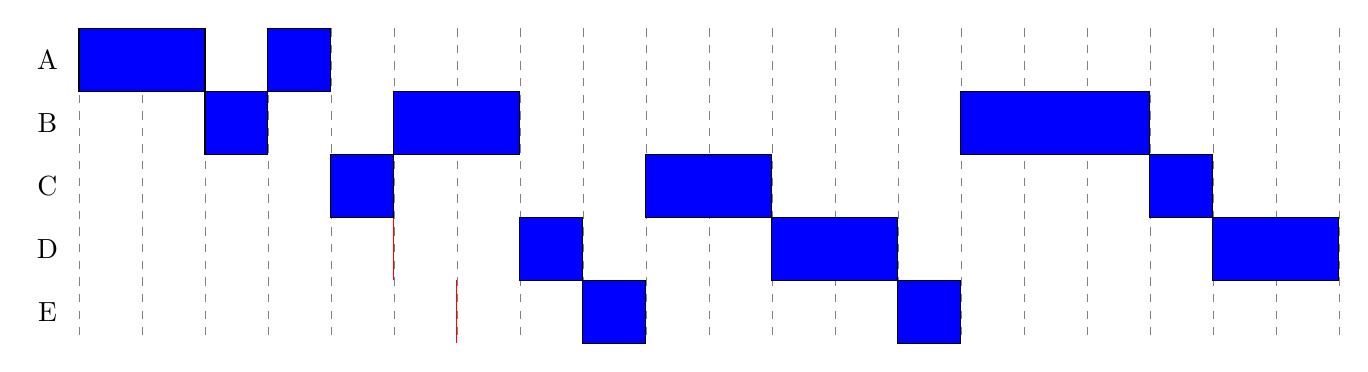
\begin{tikzpicture}[scale=.8]
   \foreach \i in {0,...,20}
   \draw[dashed, help lines] (\i,0) -- (\i,-5);

   \node (A) at (-.5,-.5) {A};
   \node (B) at (-.5,-1.5) {B};
   \node (C) at (-.5,-2.5) {C};
   \node (D) at (-.5,-3.5) {D};
   \node (E) at (-.5,-4.5) {E};

   \foreach \p in {0,...,4}
   \draw[red] (2+\p, -\p) --++ (0,-1);

   \draw[fill=blue] (0,0) rectangle (2,-1) rectangle (3,-2);
   \draw[fill=blue] (3,-1) rectangle (4,0);
   \draw[fill=blue] (4,-3) rectangle (5,-2) rectangle (7,-1);
   \draw[fill=blue] (7,-3) rectangle (8,-4) rectangle (9,-5);
   \draw[fill=blue] (9,-2) rectangle (11,-3) rectangle (13,-4) rectangle (14,-5);
   \draw[fill=blue] (14,-1) rectangle (17,-2) rectangle (18,-3) rectangle (20,-4);

\end{tikzpicture}

%Tt      4     17    18    20    14    //
%Tr      4     15    14    14    6     10.6
%Tr/Ts   4/3   15/6  14/4  14/5  6/2   2.63